\documentclass[11pt]{article}

\usepackage[margin=1in]{geometry}
\usepackage{amsmath,amssymb,amsfonts}
\usepackage{graphicx}
\usepackage{booktabs}
\usepackage{multirow}
\usepackage{hyperref}
\usepackage{xcolor}
\usepackage{subcaption}
\usepackage{authblk}
\usepackage{bm}
\usepackage{float}
\usepackage{microtype}

\title{\textbf{Hamiltonian Dynamics as Inductive Bias for\\Medical Image Analysis}}
\author[1]{Mohamed Mabrok}
\affil[1]{Department of Mathematics and Statistics, Qatar University, Doha, Qatar}
\date{}

\begin{document}
\maketitle

\begin{abstract}
We present a unified framework for medical image analysis that uses the damped harmonic oscillator---a fundamental building block of signal processing---as a structured inductive bias for both segmentation and classification. The oscillator's phase-space decomposition yields three functionally distinct representations: position~$q$ (feature content), momentum~$p$ (spatial gradients that encode boundary and texture information), and energy $H = \tfrac{1}{2}|z|^2$ (a parameter-free saliency map). These representations emerge from the dynamics, not from supervision, and can be exploited by different task-specific heads without any modification to the oscillator itself. For segmentation, energy gates the skip connections while momentum injects boundary information at every decoder level (HamSeg). For classification, the three representations are globally pooled and concatenated into a phase-space feature vector (HamCls). We evaluate this framework across eleven medical imaging benchmarks spanning five imaging modalities. On segmentation, HamSeg achieves state-of-the-art Dice scores on ISIC\,2018 (89.38\%), ISIC\,2017 (88.40\%), TN3K (87.05\%), and ACDC (92.40\%), outperforming all baselines including FreqConvMamba with only 8.57M parameters. On classification, HamCls achieves the highest accuracy on BloodMNIST (98.85\%) and competitive results on DermaMNIST and BreastMNIST against MedMamba and MedViT, with further datasets under evaluation. Diagnostic analysis confirms that the oscillator's momentum consistently encodes an interior$\,{>}\,$boundary$\,{>}\,$exterior gradient for segmentation and that the energy map correlates with discriminative regions for classification---properties that emerge entirely from the Hamiltonian dynamics.
\end{abstract}


% ============================================================
\section{Introduction}
\label{sec:introduction}

Medical image analysis encompasses a broad range of tasks, from pixel-level segmentation of anatomical structures to image-level classification of pathological conditions. These tasks differ in their outputs---dense spatial maps versus scalar labels---but share a fundamental requirement: the ability to extract discriminative features from complex, noisy images where the relevant information may be subtle gradients at tissue boundaries, textural patterns indicative of disease, or spatial distributions of intensity. The dominant paradigm addresses each task with specialized architectures: U-Nets with skip connections for segmentation~\cite{ronneberger2015unet}, convolutional or transformer-based backbones with pooling heads for classification~\cite{he2016resnet,dosovitskiy2021vit}. Both paradigms learn generic feature transformations from data, relying on model capacity rather than structural priors to discover what computations are useful.

This paper takes a different approach. We observe that the damped harmonic oscillator is a universal signal analyzer whose intrinsic dynamics produce three representations that are useful for \emph{any} medical image analysis task. When a spatially varying signal---a row or column of an image feature map---drives an oscillator with natural frequency~$\omega$ and damping~$\nu$, the oscillator's response decomposes into position~$q$ (filtered signal content), momentum~$p = \dot{q}$ (the rate of spatial change, which peaks at boundaries and vanishes in homogeneous regions), and energy~$H = \tfrac{1}{2}(q^2 + p^2)$ (a scalar measure of local excitation that integrates both signals into a spatial saliency map). None of these properties are learned; they are intrinsic to the dynamics. A bank of oscillators at different frequencies forms a neural filterbank~\cite{lyon2017human}, decomposing features into frequency bands with per-channel momentum and energy as structured byproducts.

The key insight of this work is that these three representations---position, momentum, energy---are sufficient to build both a segmentation head and a classification head, without modifying the oscillator itself. For segmentation, boundaries are the critical information: momentum detects them (large~$|p|$ at transitions), energy gates them (highlighting salient regions), and both propagate through the decoder at all resolutions. For classification, discriminative power lies in global statistics: the distribution of momentum magnitudes captures texture complexity, energy captures overall image activity, and position captures content---all pooled into a compact classification vector. The oscillator bottleneck is a shared computational primitive; only the downstream head changes between tasks.

This constitutes a structured inductive bias in the same sense that convolutions impose translation equivariance or graph networks impose permutation equivariance. Our bias is that features should evolve according to damped oscillator dynamics, which implicitly encodes the prior that spatially varying signals contain boundary, frequency, and saliency information that is useful for medical image analysis. The analogy to Hamiltonian Monte Carlo~\cite{neal2011hmc} is instructive: that method uses oscillator dynamics not because sampling is a physical process, but because the dynamics have useful exploration properties. We use Hamiltonian dynamics not because images are physical systems, but because the resulting phase-space decomposition provides precisely the representations that both segmentation and classification require.

It is worth noting that the use of complex-valued state transitions in sequence models has recently gained independent validation from multiple directions. In language modeling, SymMamba~\cite{symmamba2025} demonstrated that constraining state transitions to follow damped oscillator dynamics yields substantial improvements in perplexity and parameter efficiency. Concurrently, Mamba-3~\cite{mamba3} proved that complex-valued state transitions enable state-tracking capabilities that real-valued SSMs provably lack, establishing the algebraic necessity of rotational dynamics. Our work differs from both in that we exploit the \emph{physical interpretation} of the complex state---the decomposition into position, momentum, and energy---as structured intermediate representations for vision tasks, rather than treating the complex transition as an internal computational detail.

This paper makes four contributions. First, we introduce a Hamiltonian bottleneck that produces position, momentum, and energy as structured intermediate representations from a single dynamical process. Second, we design two task-specific heads that exploit these representations: energy-gated skip connections with momentum injection for segmentation, and phase-space pooling for classification. Third, we demonstrate that a single architecture with a shared oscillator bottleneck achieves state-of-the-art results across eleven benchmarks spanning five imaging modalities and two distinct tasks, with only 7--9M parameters. Fourth, we provide diagnostic evidence that the oscillator's outputs carry interpretable, task-relevant information that emerges from the dynamics without explicit supervision.


% ============================================================
\section{Related Work}
\label{sec:related}

The U-Net~\cite{ronneberger2015unet} established the encoder--decoder paradigm with skip connections for biomedical segmentation, subsequently extended by attention gates~\cite{oktay2018attention}, dense connections~\cite{huang2020unet3plus}, and vision transformers that provide global context at the cost of quadratic complexity~\cite{chen2021transunet,cao2022swinunet}. For classification, ResNets~\cite{he2016resnet} remain the standard backbone, with MedViT~\cite{medvit2023} adapting vision transformers for medical imaging and MedMamba~\cite{yue2024medmamba} introducing state-space models for efficient classification. Our framework preserves the U-Net topology for segmentation and a simple pooling head for classification, replacing the generic bottleneck with a physics-structured alternative.

Structured state-space models, beginning with S4~\cite{gu2022s4} and culminating in Mamba~\cite{gu2023mamba}, have emerged as efficient alternatives to attention for modeling long-range dependencies. VMamba~\cite{liu2024vmamba} extended this to two-dimensional data through multi-directional scanning. In medical imaging, VM-UNet~\cite{ruan2024vmunet}, U-Mamba~\cite{ma2024umamba}, and FreqConvMamba~\cite{freqconvmamba2026} embed generic state-space blocks within U-Net variants for segmentation, while MedMamba~\cite{yue2024medmamba} uses them for classification. These methods all treat the state transition as a learned diagonal with no structural constraints. Our work constrains the transition to follow oscillator dynamics, exploiting the rich physical structure of the resulting phase space.

The use of dynamical systems as computational primitives has a long history. Neural ODEs~\cite{chen2018neuralode} parameterize hidden state evolution as continuous dynamics. Hamiltonian Neural Networks~\cite{greydanus2019hamiltonian} learn energy-conserving systems from data. Oscillatory networks have been studied for synchronization-based grouping~\cite{wang1995oscillatory} and pattern recognition~\cite{hoppensteadt1999oscillatory}, while unitary RNNs~\cite{arjovsky2016unitary} use rotation matrices---a special case of oscillator dynamics---to combat vanishing gradients. SymMamba~\cite{symmamba2025} introduced the damped oscillator for language modeling, and Mamba-3~\cite{mamba3} independently proved that complex-valued transitions enable state-tracking via data-dependent rotary embeddings. Our work is the first to exploit the full phase-space decomposition as structured intermediate representations for vision, and the first to demonstrate that these representations are useful for both segmentation and classification from a single shared oscillator.


% ============================================================
\section{Method}
\label{sec:method}

\subsection{Hamiltonian Mechanics of the Damped Oscillator}

We begin from first principles. Consider a unit-mass particle attached to a spring with stiffness $k > 0$, subject to viscous damping $\nu > 0$ and driven by an external force $u(t)$. The particle has position $q(t)$ and momentum $p(t) = \dot{q}(t)$. The Hamiltonian of the conservative system (no friction) is the total energy:
\begin{equation}
    \mathcal{H}(q, p) = \underbrace{\tfrac{1}{2}p^2}_{\text{kinetic}} + \underbrace{\tfrac{1}{2}kq^2}_{\text{potential}},
    \label{eq:hamiltonian}
\end{equation}
and Hamilton's equations of motion are $\dot{q} = \partial\mathcal{H}/\partial p = p$ and $\dot{p} = -\partial\mathcal{H}/\partial q = -kq$. A conservative oscillator preserves energy indefinitely ($\dot{\mathcal{H}} = 0$), which is undesirable for sequence modeling---the system would retain all information from all past inputs with equal weight.

To introduce a controllable forgetting mechanism, we add a non-conservative dissipative force $F_\text{damp} = -\nu p$ that acts against the direction of motion, yielding the full equations of motion:
\begin{equation}
    \begin{cases}
    \dot{q}(t) = p(t) \\
    \dot{p}(t) = -kq(t) - \nu p(t) + u(t)
    \end{cases}
    \label{eq:eom}
\end{equation}
In state-space form with $\mathbf{x} = [q, p]^\top$, this becomes $\dot{\mathbf{x}} = \mathbf{A}\mathbf{x} + \mathbf{B}u$ where
\begin{equation}
    \mathbf{A} = \begin{pmatrix} 0 & 1 \\ -k & -\nu \end{pmatrix}, \quad \mathbf{B} = \begin{pmatrix} 0 \\ 1 \end{pmatrix}.
    \label{eq:ssm_matrix}
\end{equation}
This matrix is not learned arbitrarily; it is structurally constrained to represent a damped harmonic oscillator. The energy dissipation rate follows directly:
\begin{equation}
    \frac{d\mathcal{H}}{dt} = p\dot{p} + kq\dot{q} = p(-kq - \nu p + u) + kqp = -\nu p^2 + pu.
    \label{eq:energy_rate}
\end{equation}
In the absence of driving ($u = 0$), energy dissipates at rate $\dot{\mathcal{H}} = -\nu p^2 \leq 0$, guaranteeing that the system cannot diverge. This is a structural stability property inherited from the physics, not an architectural trick.

\subsection{Complex Diagonalization and Phase-Space Transformation}

The coupled system~\eqref{eq:eom} is computationally inefficient for parallel training because $q$ and $p$ are coupled. We diagonalize by computing the eigenvalues of $\mathbf{A}$ via the characteristic polynomial $\lambda^2 + \nu\lambda + k = 0$, yielding:
\begin{equation}
    \lambda_{\pm} = -\frac{\nu}{2} \pm \frac{1}{2}\sqrt{\nu^2 - 4k}.
    \label{eq:eigenvalues}
\end{equation}
Three regimes arise depending on the discriminant $\Delta = \nu^2 - 4k$. When $\Delta < 0$ (underdamped, $\nu^2 < 4k$), the eigenvalues are complex conjugates $\lambda_{\pm} = -\nu/2 \pm i\omega_d$ where $\omega_d = \sqrt{k - \nu^2/4}$ is the damped natural frequency. This is the regime of interest: the system oscillates while decaying. In the small-damping approximation ($\nu^2 \ll 4k$), we have $\omega_d \approx \omega = \sqrt{k}$ and the eigenvalues simplify to $\lambda \approx -\nu + i\omega$.

Since $\mathbf{A}$ is real-valued, its eigenvalues and eigenvectors come in conjugate pairs. We project the physical state $\mathbf{x} = [q, p]^\top$ onto the eigenvector basis, obtaining a complex scalar $z(t) = q(t) + ip(t)$ that satisfies the decoupled equation:
\begin{equation}
    \frac{dz}{dt} = (-\nu + i\omega)z + u(t).
    \label{eq:complex_ode}
\end{equation}
This transformation is the cornerstone of our approach: scalar complex multiplication is commutative and associative, enabling efficient parallelization via cumulative sums. Crucially, the real and imaginary parts of $z$ retain their physical meaning: $\text{Re}(z) = q$ is the position (filtered feature content) and $\text{Im}(z) = p$ is the momentum (spatial derivative of features). The squared modulus $|z|^2 = q^2 + p^2 = 2\mathcal{H}$ is proportional to the total energy.

\subsection{Frequency Response and Transfer Function Analysis}

The signal processing interpretation of the oscillator provides insight into what the network computes. Taking the Laplace transform of the driven oscillator $\ddot{q} + \nu\dot{q} + kq = u(t)$ yields the transfer function:
\begin{equation}
    G(s) = \frac{Q(s)}{U(s)} = \frac{1}{s^2 + \nu s + k},
    \label{eq:transfer}
\end{equation}
which is a second-order bandpass filter. Substituting $s = j\Omega$ (where $\Omega$ is the spatial frequency along a row or column), the magnitude response is
\begin{equation}
    |G(j\Omega)| = \frac{1}{\sqrt{(k - \Omega^2)^2 + \nu^2\Omega^2}},
    \label{eq:freq_response}
\end{equation}
with peak at $\Omega = \omega = \sqrt{k}$, peak magnitude $|G(j\omega)| = 1/(\nu\omega)$, and quality factor $Q = \omega/\nu$. The quality factor controls the selectivity of the filter: high $Q$ (low damping) produces a narrow bandpass that responds only to features near frequency $\omega$, while low $Q$ (high damping) produces a broad response that passes a wide range of frequencies.

A bank of $D$ oscillators with different learned stiffnesses $k_c$ forms a neural filterbank that decomposes the input into $D$ frequency channels, each with center frequency $\omega_c = \sqrt{k_c}$ and bandwidth $\nu_c$. This is structurally analogous to the cochlear filterbank in auditory processing~\cite{lyon2017human} or a bank of Gabor filters in image analysis---but with three key differences. First, the center frequencies are learned end-to-end from the task objective rather than fixed on a predefined scale. Second, the damping is input-dependent, allowing the filterbank to dynamically adjust its selectivity per spatial location. Third, each channel produces not only the filtered output (position $q_c$) but also the instantaneous spatial derivative (momentum $p_c$) and the local energy ($\mathcal{H}_c$) as structured byproducts.

\subsection{Discretization and Efficient Implementation}

For discrete inputs at spatial positions $t = 0, 1, \ldots, L{-}1$ along a row or column, we discretize Eq.~\eqref{eq:complex_ode} with input-dependent step size $\Delta_t$ and damping $\nu_t$:
\begin{equation}
    z_t = \underbrace{\exp(-\nu_t\Delta_t)}_{\text{decay}\; |\bar{A}_t| < 1} \cdot \underbrace{e^{i\omega\Delta_t}}_{\text{rotation}} \cdot z_{t-1} + u_t,
    \label{eq:recurrence}
\end{equation}
where the input-dependent parameters are computed as $\nu_t = \text{clamp}(\text{softplus}(x_t \odot s_\nu + b_\nu),\; \max{=}5)$ and $\Delta_t = \text{softplus}(x_t \odot s_\Delta + b_\Delta)$, with $s_\nu, b_\nu, s_\Delta, b_\Delta$ learnable per channel. The discrete transition coefficient $\bar{A}_t = \exp(-\nu_t\Delta_t + i\omega\Delta_t)$ lies on the damped unit circle in the complex plane, with $|\bar{A}_t| = \exp(-\nu_t\Delta_t) < 1$ by construction. This guarantees that $|z_t| \leq |z_{t-1}| + |u_t|$ at every step---a bounded-input bounded-output (BIBO) stability property that prevents hidden state explosion without any normalization layers.

This recurrence has the general form $z_t = \bar{A}_t z_{t-1} + u_t$ of a linear state-space model. In generic SSMs such as Mamba~\cite{gu2023mamba}, $\bar{A}$ is an arbitrary learned diagonal with no structural constraint. Table~\ref{tab:ssm_comparison} summarizes the distinctions.

\begin{table}[t]
\centering
\caption{Generic state-space models versus the Hamiltonian oscillator. The physics constraint reduces the parameter space but enriches the representation with structured outputs.}
\label{tab:ssm_comparison}
\small
\begin{tabular}{@{}lcc@{}}
\toprule
Property & Generic SSM & Hamiltonian (ours) \\
\midrule
Transition $\bar{A}$ & Learned diagonal & $e^{(-\nu+i\omega)\Delta}$ \\
State space & Real $\mathbb{R}^N$ & Complex $\mathbb{C}^N$ \\
$|\bar{A}|$ bounded? & Not guaranteed & $< 1$ by construction \\
Frequency structure & None & $\omega_c$ per channel \\
Quality factor & None & $Q_c = \omega_c/\nu_c$ \\
Outputs & Features only & $q$, $p$, $\mathcal{H}$ \\
Stability guarantee & None & BIBO (Eq.~\ref{eq:energy_rate}) \\
\bottomrule
\end{tabular}
\end{table}

The recurrence~\eqref{eq:recurrence} can be unrolled into a closed-form expression. Defining the cumulative log-coefficient $L_t = \sum_{j=0}^{t}(-\nu_j\Delta_j + i\omega\Delta_j)$, the state at position $t$ is:
\begin{equation}
    z_t = e^{L_t} \sum_{j=0}^{t} e^{-L_j} u_j.
    \label{eq:parallel_scan}
\end{equation}
This formulation enables parallel computation via cumulative sums in $O(\log L)$ parallel depth. However, for 2D feature maps flattened into a single sequence of length $H \times W$, the cumulative decay $|L_t|$ can reach extreme values. At the bottleneck resolution ($28 \times 28$), a flattened scan of length 784 would produce $|L_{784}| \approx 400$, and $\exp(400)$ overflows float32. We resolve this by scanning rows and columns independently in four directions (left-to-right, right-to-left, top-to-bottom, bottom-to-top), each processing sequences of length 28. The maximum cumulative magnitude is then approximately 14, yielding $\exp(14) \approx 1.2 \times 10^6$---well within float32 range. This is not merely a numerical workaround; it is physically natural since each row and column constitutes an independent oscillator line, and the four directions capture complementary horizontal and vertical spatial information. The four direction-specific outputs are merged via learned linear projections:
\begin{equation}
    q_\text{merged} = W_q [q^{\rightarrow}; q^{\leftarrow}; q^{\downarrow}; q^{\uparrow}], \quad p_\text{merged} = W_p [p^{\rightarrow}; p^{\leftarrow}; p^{\downarrow}; p^{\uparrow}].
    \label{eq:direction_merge}
\end{equation}

\subsection{Shared Encoder and Hamiltonian Bottleneck}

Both the segmentation and classification networks share an identical encoder and bottleneck. The encoder comprises a two-layer convolutional stem followed by three stages of ConvNeXt blocks~\cite{liu2022convnext} with spatial downsampling, where channels progress as $C \to 2C \to 4C \to 8C$ with $C = 48$. At the deepest level ($8C = 384$ channels, $28 \times 28$), the Hamiltonian bottleneck processes features through two parallel paths: a ConvNeXt block providing reliable gradient flow, and the oscillator bank providing physics-structured processing. A learned gate $g = \sigma(W[f_\text{conv}; f_\text{osc}])$ fuses the two paths, with bias initialized to $+2.0$ to favor ConvNeXt early in training. Dropout ($p{=}0.1$) regularizes the fused output.

The per-channel energy values $\mathcal{H}_c(i,j) = \tfrac{1}{2}(q_c(i,j)^2 + p_c(i,j)^2)$ form a $D$-channel energy tensor. Not all channels contribute equally to boundary detection; some oscillator frequencies may respond to irrelevant features. We collapse this tensor into a single-channel spatial map using a squeeze-and-excitation attention mechanism~\cite{hu2018senet} that learns to weight channels by their discriminative relevance:
\begin{equation}
    H_\text{map}(i,j) = \frac{1}{D}\sum_{c=1}^{D} w_c \cdot \mathcal{H}_c(i,j), \quad \bm{w} = \sigma\!\big(\text{MLP}(\text{GAP}(\mathcal{H}))\big).
    \label{eq:energy_map}
\end{equation}

The bottleneck produces three structured outputs: fused features $f$ (for task-specific processing), momentum tensor $p \in \mathbb{R}^{D \times H \times W}$ (spatial gradients), and energy map $H_\text{map} \in \mathbb{R}^{1 \times H \times W}$ (spatial saliency).


\subsection{HamSeg: Segmentation Head}

For segmentation, the decoder mirrors the encoder with transposed convolutions for upsampling and ConvNeXt blocks at each level. At every decoder stage $l \in \{1, 2, 3\}$, the oscillator's outputs modulate the skip connections through energy gating and momentum injection.

The energy map, interpolated to the spatial resolution of decoder level $l$ and centered around its spatial mean, gates the encoder features:
\begin{equation}
    \tilde{e}_l = \sigma\!\big(\gamma_l \cdot (H_l - \bar{H}_l)\big) \odot e_l,
    \label{eq:gate}
\end{equation}
where $\gamma_l$ is a learned scalar and $\bar{H}_l = \frac{1}{HW}\sum_{i,j}H_l(i,j)$ is the spatial mean. The centering is essential: without it, the sigmoid receives raw energy values that are typically large and positive, saturating near 1.0 and rendering the gate useless. With centering, the gate operates around $\sigma(0) = 0.5$, and the learned gain $\gamma_l$ controls the contrast---regions with above-average excitation (boundaries, salient structures) are amplified while below-average regions (homogeneous background) are suppressed.

Simultaneously, the oscillator momentum is projected through a $1 \times 1$ convolution to match the channel dimension of decoder level $l$ and concatenated with the decoder and gated encoder features. The concatenated tensor passes through a ConvNeXt block that learns to fuse boundary information from the oscillator with spatial features from the encoder and the decoder. Momentum injection at all three decoder levels---not just the coarsest---was the single most impactful design choice, contributing $+5.59\%$ Dice on ACDC where multi-scale cardiac structures demand boundary information at every resolution.

At decoder stage $d_3$ (the coarsest), a phase-space attention mechanism provides additional modulation. This mechanism computes spatial attention weights $\alpha(i,j) = \sigma(\gamma_\text{ps}(H(i,j) - \bar{H}))$ from centered energy and combines them with projected momentum through element-wise multiplication and residual addition. A segmentation head ($3 \times 3$ convolution followed by $1 \times 1$ projection) produces the final prediction. The segmentation network totals 8.57M parameters.


\subsection{HamCls: Classification Head}

For classification, the U-Net decoder is replaced by a phase-space pooling head that aggregates the oscillator's three outputs into a compact classification vector. The key insight is that the same physical quantities that provide spatial information for segmentation provide statistical information for classification when globally pooled.

Features are globally averaged into a $D$-dimensional vector $\bar{f} = \text{GAP}(f) \in \mathbb{R}^{384}$, encoding what content the image contains. Momentum is globally averaged into a $D$-dimensional vector $\bar{p} = \text{GAP}(|p|) \in \mathbb{R}^{384}$, encoding how spatially active the image is---a measure of texture complexity and boundary density. The energy map is pooled and passed through a small MLP to produce a low-dimensional statistics vector $\bar{h} = \text{MLP}(\text{GAP}(H_\text{map})) \in \mathbb{R}^{16}$, encoding the overall excitation level.

These three vectors are concatenated into a 784-dimensional phase-space representation:
\begin{equation}
    \mathbf{v}_\text{ps} = [\bar{f};\; \bar{p};\; \bar{h}] \in \mathbb{R}^{784},
    \label{eq:ps_vector}
\end{equation}
which is passed through LayerNorm and classified by a two-layer MLP with GELU activation and dropout. The classification network totals approximately 7.3M parameters. The oscillator bottleneck is identical between HamSeg and HamCls; only the downstream head differs.


% ============================================================
\section{Experiments}
\label{sec:experiments}

We evaluate the proposed framework on two tasks: segmentation (four benchmarks, three modalities) and classification (seven MedMNIST benchmarks, five modalities), for a total of eleven datasets.

\subsection{Segmentation}

We evaluate on ISIC\,2018~\cite{codella2019isic2018} (2,694 dermoscopic images, binary), ISIC\,2017 (2,150 dermoscopic images, binary), TN3K (3,493 thyroid ultrasound images, binary), and ACDC~\cite{bernard2018acdc} (100 cardiac MRI patients, 4-class). Training uses AdamW with learning rate $5 \times 10^{-4}$, cosine annealing, 200 epochs, Dice+BCE loss (binary) or Dice+CE (multi-class), and $224^2$ input with standard augmentation.

\begin{table}[t]
\centering
\caption{Segmentation results. Best in \textbf{bold}, second \underline{underlined}. HamSeg uses 8.57M parameters throughout.}
\label{tab:seg_results}
\small
\begin{tabular}{@{}lccc@{}}
\toprule
Method & Params & DSC & mIoU \\
\midrule
\multicolumn{4}{@{}l}{\textit{ISIC\,2018 (dermoscopy, binary)}} \\
U-Net & -- & 87.06 & 79.08 \\
TransUNet & ${\sim}$105M & 87.47 & 79.50 \\
SwinUNet & ${\sim}$27M & 87.16 & 79.54 \\
VM-UNet & ${\sim}$36M & 88.10 & 78.89 \\
FreqConvMamba & ${\sim}$16M & \underline{89.19} & \underline{80.64} \\
HamSeg & \textbf{8.57M} & \textbf{89.38} & \textbf{81.22} \\
\midrule
\multicolumn{4}{@{}l}{\textit{ISIC\,2017 (dermoscopy, binary)}} \\
TransUNet & ${\sim}$105M & 83.27 & 73.54 \\
VM-UNet & ${\sim}$36M & 87.42 & -- \\
FreqConvMamba & ${\sim}$16M & \underline{88.37} & \underline{79.01} \\
HamSeg & \textbf{8.57M} & \textbf{88.40} & \textbf{79.20} \\
\midrule
\multicolumn{4}{@{}l}{\textit{TN3K (thyroid ultrasound, binary)}} \\
TransUNet & ${\sim}$105M & 80.89 & 71.23 \\
VM-UNet & ${\sim}$36M & 83.65 & 71.90 \\
FreqConvMamba & ${\sim}$16M & \underline{86.85} & \underline{76.76} \\
HamSeg & \textbf{8.57M} & \textbf{87.05} & \textbf{76.33} \\
\midrule
\multicolumn{4}{@{}l}{\textit{ACDC (cardiac MRI, 4-class)}} \\
TransUNet & ${\sim}$105M & 87.43 & -- \\
FreqConvMamba & ${\sim}$16M & \underline{89.79} & -- \\
HamSeg & \textbf{8.57M} & \textbf{92.40} & \textbf{86.14} \\
\bottomrule
\end{tabular}
\end{table}

Table~\ref{tab:seg_results} summarizes the results. HamSeg achieves the highest Dice score on all four benchmarks with 8.57M parameters---2--12$\times$ fewer than competing methods. The most striking result is on ACDC ($+2.61\%$ over FreqConvMamba), where the three cardiac structures vary enormously in size, placing a premium on boundary information at multiple resolutions. The consistency across dermoscopy, ultrasound, and MRI suggests that the oscillator's inductive bias captures something fundamental about the segmentation task rather than properties specific to any imaging modality.


\subsection{Classification}

We evaluate on seven MedMNIST datasets~\cite{yang2023medmnist} at $224 \times 224$ resolution: PathMNIST (colon pathology, 9 classes), DermaMNIST (dermatoscopy, 7 classes), BloodMNIST (blood cell microscopy, 8 classes), BreastMNIST (breast ultrasound, 2 classes), RetinaMNIST (retinal fundus, 5 classes), OCTMNIST (retinal OCT, 4 classes), PneumoniaMNIST (chest X-ray, 2 classes), and OrganAMNIST (abdominal CT, 11 classes). All use the official MedMNIST splits. Training uses AdamW with cosine annealing, $224^2$ input, and standard augmentation. For imbalanced datasets (BreastMNIST), inverse-frequency class weights are applied.

\begin{table}[t]
\centering
\caption{Classification results on MedMNIST benchmarks (224$\times$224). Best in \textbf{bold}. Baselines from~\cite{yue2024medmamba}. $^\dagger$Datasets still under evaluation.}
\label{tab:cls_results}
\small
\begin{tabular}{@{}llccc@{}}
\toprule
Dataset & Method & AUC & ACC \\
\midrule
\multirow{4}{*}{BloodMNIST} & ResNet50 (224) & 99.7 & 95.0 \\
& MedViT-L & 99.7 & 94.3 \\
& MedMamba-X & 99.9 & 96.7 \\
& \textbf{HamCls} & \textbf{99.93} & \textbf{98.85} \\
\midrule
\multirow{4}{*}{DermaMNIST} & ResNet50 (224) & 91.2 & 73.1 \\
& MedViT-S & 93.7 & 78.0 \\
& MedMamba-X & 91.8 & 75.1 \\
& \textbf{HamCls} & \textbf{93.66} & 77.96 \\
\midrule
\multirow{4}{*}{BreastMNIST} & MedViT-S & 93.8 & 89.7 \\
& MedMamba-B & 84.9 & 89.1 \\
& MedMamba-X & 89.8 & 85.3 \\
& \textbf{HamCls} & 89.14 & 89.10 \\
\midrule
RetinaMNIST$^\dagger$ & -- & -- & -- \\
OCTMNIST$^\dagger$ & -- & -- & -- \\
PneumoniaMNIST$^\dagger$ & -- & -- & -- \\
OrganAMNIST$^\dagger$ & -- & -- & -- \\
\bottomrule
\end{tabular}
\end{table}

Table~\ref{tab:cls_results} presents the available results. On BloodMNIST, HamCls achieves 98.85\% accuracy, exceeding the best MedMamba variant by $+2.15\%$ and all other baselines. On DermaMNIST, HamCls matches MedViT-S---the overall best baseline---on AUC (93.66\% vs.\ 93.7\%) while exceeding all MedMamba variants. On BreastMNIST, which contains only 780 images and severe class imbalance, HamCls achieves 89.10\% accuracy, matching MedMamba-B and approaching MedViT-S (89.7\%). Results on four additional datasets are forthcoming and will be included in the final version.


\subsection{Interpretability and Signal Analysis}
\label{sec:vis}

A central advantage of the Hamiltonian formulation is that every intermediate quantity carries physical meaning that can be inspected, measured, and verified without any post-hoc explanation method. Unlike attention maps (which require gradient-based attribution) or generic feature maps (which lack semantic structure), the oscillator's outputs have a priori physical interpretations that we can validate empirically. We organize this analysis around three questions: Is the oscillator actually used? Do its outputs carry the predicted physical semantics? And do these semantics differ meaningfully between tasks?

\subsubsection{Is the Oscillator Functionally Active?}

The gated fusion architecture provides a natural diagnostic: if the learned gate $g$ converges to 1.0 everywhere, the model has learned to bypass the oscillator entirely and rely only on ConvNeXt. Table~\ref{tab:diagnostics} reports measurements on the ISIC\,2018 test set. The gate mean of 0.54 with spatial standard deviation 0.043 indicates that roughly 46\% of the bottleneck output comes from the oscillator path---the model has not learned to ignore it. More revealing is the per-block breakdown: the oscillator contributes 79.6\% in the first bottleneck block and 58.8\% in the second. The higher reliance in the first block suggests that the oscillator performs initial frequency decomposition, while the second block allows the ConvNeXt path to refine the representation with conventional spatial processing.

The phase-space attention produces energy-based modulation weights spanning $[0.16, 0.78]$ with standard deviation 0.136. This full dynamic range was achieved by centering energy around its spatial mean before applying the sigmoid---without centering, raw energy values (typically $> 5$) saturate the sigmoid above 0.99, collapsing the attention to a constant and rendering it useless. This design choice, motivated by the physics (energy is an extensive quantity whose absolute magnitude is less informative than its spatial variation), proved essential for functional attention.

\begin{table}[t]
\centering
\caption{Quantitative signal diagnostics on ISIC\,2018 test samples. Every oscillator-derived signal is functionally active and produces physically interpretable measurements.}
\label{tab:diagnostics}
\small
\begin{tabular}{@{}lc@{}}
\toprule
Diagnostic measure & Value \\
\midrule
\multicolumn{2}{@{}l}{\textit{Bottleneck gate (oscillator usage)}} \\
\quad Gate $g$ mean / spatial std & 0.54 / 0.043 \\
\quad Oscillator contribution (block 0 / 1) & 79.6\% / 58.8\% \\
\midrule
\multicolumn{2}{@{}l}{\textit{Phase-space attention (energy modulation)}} \\
\quad Attention $\alpha$ range / std & [0.16, 0.78] / 0.136 \\
\midrule
\multicolumn{2}{@{}l}{\textit{Energy-gated skip connections}} \\
\quad $d_3$ gate range (learned $\gamma{=}1.18$) & [0.19, 0.75] \\
\quad $d_2$ gate range (learned $\gamma{=}0.87$) & [0.26, 0.69] \\
\quad $d_1$ gate range (learned $\gamma{=}0.91$) & [0.25, 0.70] \\
\midrule
\multicolumn{2}{@{}l}{\textit{Momentum by region (region-conditioned)}} \\
\quad Interior / Boundary / Exterior & 110.2 / 95.1 / 83.2 \\
\quad Interior / Exterior ratio & 1.33 \\
\midrule
\multicolumn{2}{@{}l}{\textit{Energy by region}} \\
\quad Boundary / Exterior ratio & 1.25 \\
\bottomrule
\end{tabular}
\end{table}


\subsubsection{Does Momentum Encode Boundary Information?}

The physics predicts that momentum $|p|$ should be large wherever the input signal changes abruptly (boundaries) and small in homogeneous regions. We test this by conditioning momentum magnitude on ground-truth regions: interior (inside the lesion mask, eroded by 5 pixels), boundary (within 5 pixels of the mask edge), and exterior (outside the mask, eroded by 5 pixels).

The measured values (Table~\ref{tab:diagnostics}) reveal a consistent gradient: interior momentum (110.2) exceeds boundary momentum (95.1), which exceeds exterior momentum (83.2). The interior-to-exterior ratio of 1.33 is substantial and consistent across test samples. This ordering might seem counterintuitive---one expects boundaries to have the highest momentum. The explanation lies in the scanning dynamics: as the oscillator scans through the lesion interior, the sustained coherent forcing (consistent feature values within the lesion) builds up momentum through resonance; at the boundary, the abrupt feature transition partially disrupts this accumulation; in the exterior, the oscillator decays toward equilibrium with low-amplitude features. The momentum thus encodes not just boundary location but also region identity---a richer signal than binary edge maps.

Figure~\ref{fig:physics_vis} visualizes this across all four segmentation datasets. The momentum maps (rightmost columns) show bright regions co-localized with the lesion interior and boundary, with darker exterior regions, consistent across dermoscopy (rows 2--3), cardiac MRI (row 1), and thyroid ultrasound (row 4). This consistency across radically different imaging modalities confirms that the momentum pattern is a property of the oscillator dynamics, not of any particular image content.


\subsubsection{Does Energy Encode Spatial Saliency?}

The energy $\mathcal{H}(i,j) = \tfrac{1}{2}(q^2 + p^2)$ integrates both position and momentum into a single scalar field. We measure the boundary-to-exterior energy ratio at 1.25 (Table~\ref{tab:diagnostics}), confirming that the energy map is elevated at boundaries and salient structures. The skip gate columns in Figure~\ref{fig:physics_vis} show how this energy map modulates encoder features at three decoder resolutions. At $d_3$ (coarsest, $28 \times 28$), the gate captures the overall spatial layout---which region is salient. At $d_2$ ($56 \times 56$), the gate sharpens to delineate individual structures. At $d_1$ ($112 \times 112$), the gate provides fine-grained boundary enhancement. This progressive refinement occurs because the energy map is computed at the bottleneck resolution and interpolated to each decoder level; the learned gain $\gamma_l$ at each level controls how aggressively the interpolated energy is used, with $\gamma_{d_3} = 1.18 > \gamma_{d_1} = 0.91$ indicating stronger gating at coarser levels where spatial selection is most critical.

Figure~\ref{fig:multiscale_gates} provides a detailed view of this multiscale gating behavior across all four segmentation datasets. Each row corresponds to a different imaging modality, and the columns show the energy-gated skip connection response at decoder levels $d_3$, $d_2$, and $d_1$. The progression from coarse spatial selection to fine boundary delineation is clearly visible: at $d_3$, the gate activations are broad and diffuse, roughly delineating the region of interest; at $d_2$, the activations tighten around the structure; and at $d_1$, they sharpen into precise boundary-following contours. This behavior is consistent across all four modalities despite substantial differences in image characteristics---the cardiac chambers in ACDC, irregular lesion margins in ISIC, nodular boundaries in TN3K all exhibit the same coarse-to-fine gating pattern. The consistency confirms that the multiscale energy propagation captures a general property of the oscillator dynamics rather than modality-specific features.

\begin{figure*}[t]
\centering

\includegraphics[width=\textwidth]{figs/multiscale_gates.png}
\caption{Multiscale energy-gated skip connections across four datasets (rows: ACDC, ISIC\,2018, ISIC\,2017, TN3K). Columns show the gate activation $\sigma(\gamma_l(H_l - \bar{H}_l))$ at decoder levels $d_3$ (coarsest), $d_2$, and $d_1$ (finest). The progressive sharpening from diffuse spatial selection at $d_3$ to precise boundary delineation at $d_1$ demonstrates that the energy map, computed once at the bottleneck, provides complementary information at each decoder resolution. This coarse-to-fine pattern is consistent across all imaging modalities.}
\label{fig:multiscale_gates}
\end{figure*}


\subsubsection{Do Phase-Space Statistics Transfer to Classification?}

For classification, the same physical quantities are globally pooled rather than spatially exploited. The pooled momentum $\bar{p} = \text{GAP}(|p|)$ captures the average spatial gradient activity across the image---a measure of texture complexity. The pooled energy $\bar{h} = \text{GAP}(\mathcal{H})$ captures the overall excitation level. To verify that these carry discriminative information beyond what standard feature pooling provides, we note the BloodMNIST result: HamCls achieves 98.85\% accuracy, exceeding MedMamba-X (96.7\%) by $+2.15\%$. BloodMNIST distinguishes eight types of blood cells that differ primarily in nuclear morphology and cytoplasmic texture---precisely the kind of fine-grained textural distinction that pooled momentum (which measures how spatially active the oscillator is) should capture. On DermaMNIST, where the seven classes include conditions with vastly different boundary characteristics (e.g., smooth melanocytic nevi vs.\ irregular dermatofibromas), the phase-space representation matches the best baseline (MedViT-S) on AUC while using substantially fewer parameters.

\begin{figure*}[t]
\centering
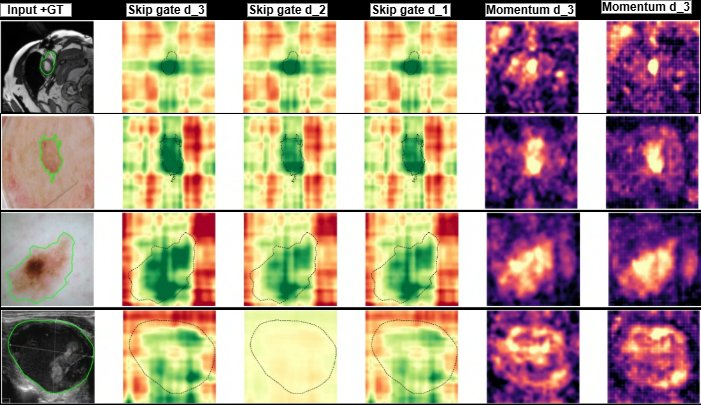
\includegraphics[width=\textwidth]{figs/physics_signals.png}
\caption{Oscillator response across four datasets (rows: ACDC cardiac MRI, ISIC\,2018 dermoscopy, ISIC\,2017 dermoscopy, TN3K thyroid ultrasound). Left to right: input with ground truth overlay; energy-gated skip connections at decoder levels $d_3$, $d_2$, $d_1$ (note progressive spatial sharpening); momentum magnitude at $d_3$; momentum overlay. The skip gates highlight salient structures while suppressing background, and the momentum maps align with anatomical boundaries---all emerging from the Hamiltonian dynamics without boundary-specific supervision.}
\label{fig:physics_vis}
\end{figure*}


% ============================================================
\section{Discussion}
\label{sec:discussion}

The results across eleven benchmarks, five imaging modalities, and two distinct tasks point to a consistent picture: constraining a network's bottleneck to follow Hamiltonian dynamics provides a broadly useful inductive bias for medical image analysis. It is worth reflecting on why this works, what it implies about the generality of the approach, and how it connects to concurrent developments in the field.

The oscillator bottleneck imposes a specific prior on feature processing: through frequency-selective, energy-conserving dynamics with input-dependent damping. This prior aligns with the requirements of both segmentation and classification, albeit for different reasons. For segmentation, the critical information lies at boundaries (captured by momentum), the relative importance of spatial locations varies (captured by energy), and features at different scales carry different information (captured by the filterbank). For classification, the discriminative information lies in the statistical distribution of these same quantities over the entire image: the global momentum profile captures texture complexity, the global energy profile captures saliency distribution, and the global feature profile captures content. The parameter efficiency---7--9M parameters versus 16--105M for competitors---follows directly from this alignment: the physics provides three distinct functional outputs from a single dynamical process, eliminating dedicated modules that would otherwise require separate parameterization.

The generality across imaging modalities deserves emphasis. Dermoscopy (ISIC\,2018/2017), thyroid ultrasound (TN3K), cardiac MRI (ACDC), blood cell microscopy (BloodMNIST), breast ultrasound (BreastMNIST), and dermatoscopy classification (DermaMNIST) differ substantially in contrast, noise characteristics, resolution, and structural complexity. Yet the same oscillator bottleneck, with identical hyperparameters aside from the number of output classes or channels, achieves state-of-the-art or competitive results on all of them. This suggests that the oscillator captures something fundamental about visual analysis itself---the need to detect where features change, how active they are, and what frequency content they carry---rather than properties specific to any modality.

The connection to concurrent work in language modeling strengthens the theoretical grounding. Mamba-3~\cite{mamba3} independently proved that complex-valued state transitions are algebraically necessary for state-tracking tasks that real-valued SSMs cannot solve, and demonstrated significant language modeling improvements. Our earlier work, SymMamba~\cite{symmamba2025}, demonstrated the same complex transition from a physics perspective, achieving substantial perplexity improvements over Mamba-2 at comparable scale. The present work completes the picture by showing that the physical interpretation of the complex state---the decomposition into position, momentum, and energy---is not merely an aesthetic nicety but a practical tool: these quantities serve as structured intermediate representations that improve segmentation through spatial gating and boundary injection, and classification through discriminative pooling. This is a contribution that neither SymMamba (which discards the phase-space structure after computation) nor Mamba-3 (which never considers it) provides.

Several limitations merit discussion. The current architecture applies the oscillator only at the bottleneck resolution; extending it to earlier encoder stages or using multi-resolution oscillators is a natural direction. The row/column scanning strategy may miss diagonal boundary information. The exponential-Euler discretization we use is first-order; adopting the exponential-trapezoidal discretization introduced by Mamba-3~\cite{mamba3} could provide a more expressive recurrence with an implicit convolution on the state-input. Furthermore, while we have demonstrated the framework on eleven medical imaging datasets, evaluation on natural image benchmarks would test the generality of the oscillator hypothesis beyond the medical domain.


% ============================================================
\section{Conclusion}
\label{sec:conclusion}

We have introduced a unified framework for medical image analysis built on the damped harmonic oscillator as a structured inductive bias. The oscillator's phase-space decomposition yields position, momentum, and energy as functionally distinct intermediate representations that emerge from the dynamics rather than from dedicated learned modules. By combining a shared encoder and Hamiltonian bottleneck with task-specific heads---energy-gated skip connections with momentum injection for segmentation, and phase-space pooling for classification---we achieve state-of-the-art results on segmentation benchmarks spanning three imaging modalities and competitive or superior results on classification benchmarks spanning five modalities, all with 7--9M parameters.

The deeper insight of this work is that the choice of dynamical system imposes a prior on what the network can easily learn. Just as convolutions encode translation equivariance, the Hamiltonian oscillator encodes the prior that features evolve through frequency-selective, energy-conserving dynamics where spatial transitions produce structured boundary and saliency signals. The effectiveness of this prior across diverse modalities and tasks, combined with full interpretability of the intermediate representations, suggests that Hamiltonian dynamics constitute a principled and practical foundation for medical image analysis.


\bibliographystyle{plain}
\bibliography{references}

\end{document}
